
% manuscript, to be drafted

%%This is a very basic article template.
%%There is just one section and two subsections.
%\documentclass[12pt,oneside,a4paper,doublespacing]{article} % for submission
\documentclass[11pt,oneside,a4paper]{article} % for sharing

\usepackage{appendix}
\usepackage{amsmath}
\usepackage{caption}
\usepackage{placeins}
\usepackage{graphicx}
\usepackage{subcaption}
%\usepackage{subfig}
\usepackage{longtable}
\usepackage{setspace}
%\usepackage{tikz}
\usepackage{booktabs}
\usepackage{tabularx}
\usepackage{xcolor,colortbl}
\usepackage{chngpage}
%\usepackage[active,tightpage]{preview}
\usepackage{natbib}
\bibpunct{(}{)}{,}{a}{}{;} 
\usepackage{url}
\usepackage{nth}
\usepackage{authblk}
\usepackage[most]{tcolorbox}
%\usepackage{hyperref}
%\usepackage{color}
%\usepackage{fontspec}
%\usepackage{pdfsync}
\usepackage[normalem]{ulem}
\usepackage{amsfonts}
\usepackage{xfrac}
%\renewcommand{\listtablename}{List of Appendix Tables}
%\newcolumntype{C}[1]{>{\centering\let\newline\\\arraybackslash\hspace{0pt}}m{#1}}
%\newcolumntype{L}[1]{>{\raggedright\let\newline\\\arraybackslash\hspace{0pt}}m{#1}}
% working on this need to concatenate file name based on sex and variable name
%\newcommand\Cell[1]{{\raisebox{-0.05in}{\includegraphics[height=.2in,width=.2in]{Figures/ColorCodes/\expandafter#1}}}}  

%%%%%%%%%%%%%%%%%%%%%%%%%%%%%%%%%%%%%%%%%%%%%%%%%%%%%%%%%%%%%%%%%%%%%%%%%%%%%
% setting color to letters affects spacing. Here's a hack I found here:
% http://tex.stackexchange.com/questions/212736/change-letter-colour-without-losing-letter-spacing
%\DeclareRobustCommand{\spacedallcaps}[1]{\MakeUppercase{\textsc{#1}}} % all
% caps with better spacing

%\colorlet{RED}{red}
%\colorlet{BLUE}{b}
%\colorlet{rd}{red}
%\colorlet{bl}{blue}

%%%%%%%%%%%%%%%%%%%%%%%%%%%%%%%%%%%%%%%%%%%%%%%%%%%%%%%%%%%%%%%%%%%%%%%%%%%%%%

\newcommand\ackn[1]{%
  \begingroup
  \renewcommand\thefootnote{}\footnote{#1}%
  \addtocounter{footnote}{-1}%
  \endgroup
}
%\newcommand\vt[1]{\textcolor{rd}{#1}}
%\newcommand\eg[1]{\textcolor{bl}{#1}}

%\newcommand\tg[1]{\includegraphics[scale=.5]{Figures/triadtable/triad#1.pdf}}
%\newcommand\tgh[1]{\raisebox{-.25\height}{\includegraphics[scale=.3]{Figures/triadtable/triad#1.pdf}}}

\defcitealias{HMD}{HMD}
\newcommand{\dd}{\; \mathrm{d}}
\newcommand{\tc}{\quad\quad\text{,}}
\newcommand{\tp}{\quad\quad\text{.}}
% junk for longtable caption
\AtBeginEnvironment{longtable}{\linespread{1}\selectfont}
\setlength{\LTcapwidth}{\linewidth}

%%%%%%%%%%%%%%%%%%%%%%%%%%%%%%%
\begin{document}

\title{Incorporating time-to-death processes in age-structured prevalence
models}

\author[1]{Tim Riffe}
%\author[3]{John MacInnes}
\affil[1]{Max Planck Institute for Demographic Research}
%\affil[2]{Department of Demography, University of California, Berkeley}
%\affil[3]{School of Social and Political Science, University of Edinburgh}

%\author{[Authors]}

\maketitle


\section{Morbidity as a function of time-to-death}
 
 Some morbidity conditions vary as a function of time to death much more than as
 a function of age itself \citep{riffe2015ttd}. For such conditions, the
 age-pattern (Sulivan curve) is itself a function of both mortality and the
 time-to-death pattern of the condition. That is to say, changing mortality will
 change the Sullivan curve independently of changes in the time-to-death
 process. As Hal mentioned, morbidity projections are often made assuming a
 fixed Sullivan curve. Such projections usually force improving mortality. When
 morbidity is assumed fixed, a projection based on the Sullivan curve will
 deviate non-trivially from a projection based on the time-to-death pattern of
 the same morbidity condition. It is straightforward to describe this phenomenon
 in continuous math, but it was my goal to implement the underlying calculations
 for the resulting health expectancies using matrices. I have used a combination
 of real matrix calculus and cheap hacks to attain this goal.
 
 \section{Method}
 
 Rather than embed the time-to-death process in a much-expanded transition
 matrix and matching reward matrix, I proceed by making the age pattern of
 prevalence a function of time-to-death, prior to creation of the rewards
 matrix. This is a cheap workaround for the sake of results.
 
 Say we have a time to death pattern of prevalence, $g(y)$, something like this:
 % Figure\ref{fig:gy}
 \begin{figure}
	\centering
	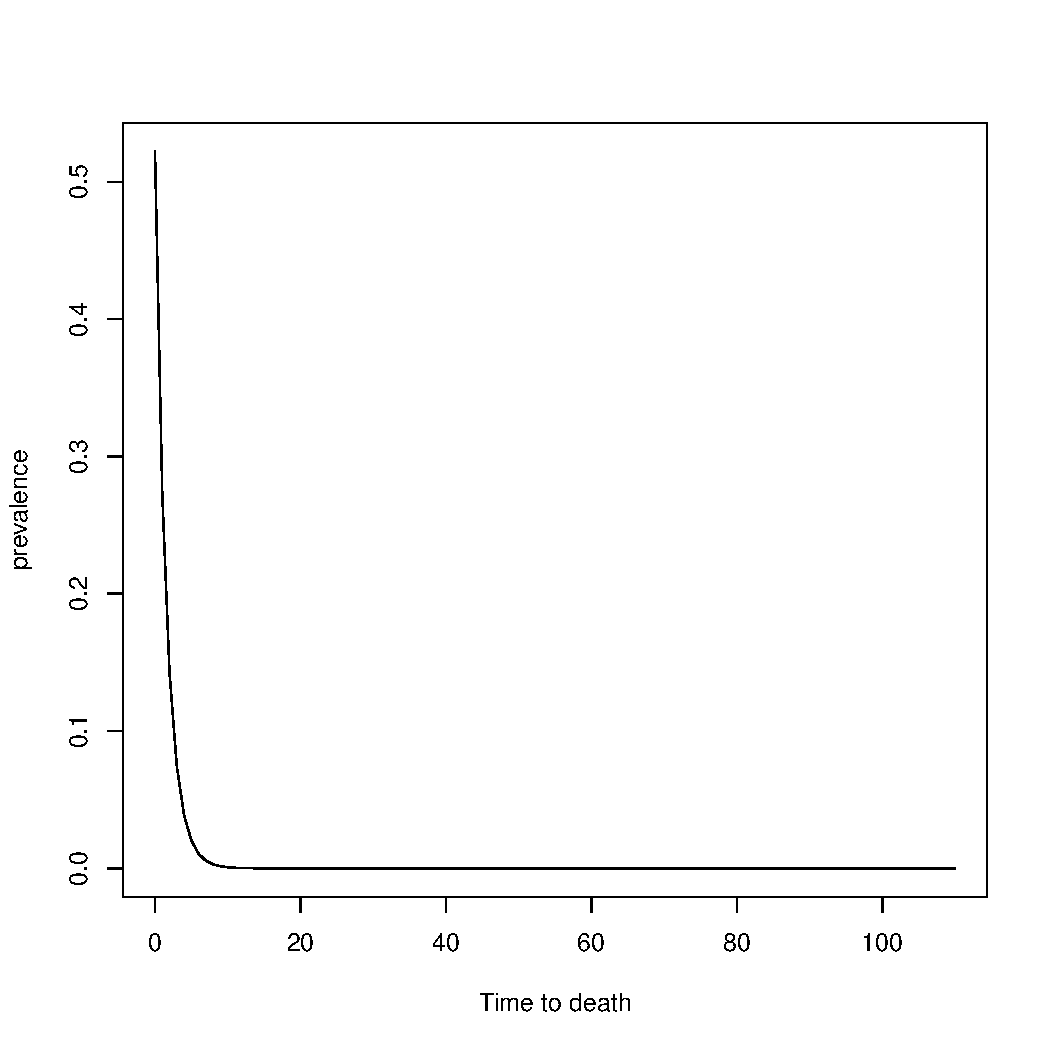
\includegraphics[scale=.7]{Figures/gyTim.pdf}
	\caption{A fake time-to-death process}
	\label{fig:gy}
\end{figure}
Prevalence is essentially zero until very close to death, where it accelerates
rapidly. 

Matrix calculations proceed by manipulating an object created by what is
possibly one of the coolest tricks I learned in Hal's course. Recall the matrix,
\textbf{N}, created by taking the inverse of the matrix that contains
conditional death probabilities in the subdiagonal. Understanding the
demographic interpretation of \textbf{N} is key: Each column of \textbf{N} gives
the conditional remaining survival curve, identical to $\frac{l(x+y)}{l(x)}$.
That a matrix inverse can produce for us this useful and meaningful object is black
magic to me, but we will exploit it.

We need to do two basic things to \textbf{N} in order to make progess: First, we
need a matrix of the condtional remaining lifespan distribution, \textbf{D},
rather than the conditional survival curve. This is just negative the first row difference of \textbf{N},
or (roughly):

\begin{equation}
\text{\textbf{D}}(m, i) = \text{\textbf{N}}(m, i) 
- \text{\textbf{N}}(m+1, i)
\end{equation}
note, you need to append a row of zeros to \textbf{N} before this in order to
close out the lifetable and ensure that the dimensions of \textbf{D} are
identical to \textbf{N}. Since the subdiagonal of \textbf{N} was 1 before, and
the upper triangle of \textbf{N} is populated with zeros, we get a -1 in the
diagonal of \textbf{D}. We can erase this by taking the Hadamard product of
\textbf{D} with the lower triangle matrix of \textbf{D} (not inclusive of the
diagonal).
\begin{equation}
\mathcal{D} = \text{\textbf{D}} \odot lower(\text{\textbf{D}})
\end{equation}
You could get the same result by populating the upper triangle of \textbf{N}
with 1s and then just taking minus the row differences\ldots

Now we have \textbf{D}, where each column contains the conditional remaining
lifetime distribution, or $\frac{d(x+y)}{l(x)}$, so we have the numbers we need,
but they're in the the wrong places in the matrix for multiplying! Note, we have
values descending down columns starting from the matrix diagonal. The diagonal
is now interpreted as zero remaining years of life, and the subdiagonal means 1
remaining year of life, and so forth. We want all ``zero remaining years'' to be
in the same row, and all the ``one remaining year'' to be in the next row, and
so forth. That is to say the lower triangle needs to ``lift'' to the top of the
matrix, leaving zeros below it. We'll call this matrix $\mathcal{D}^{up}$.
This is not the same as a simple transpose, and it was the crux of this problem\ldots

First take $vec(\mathcal{D})$, which is easy to program. Now define the
$vec^{-1}$ function, which let's us jump back to a matrix from a vector
\begin{equation}
vec^{-1}(vec(\mathcal{D})) =\mathcal{D} 
\end{equation}

Our goal is to create the matrix $\mathcal{D}^{up}$ from $\mathcal{D}$ via first
turning  $\mathcal{D}$ into a vector, then permuting its positions, then
reforming to $\mathcal{D}^{up}$ via the $vec^{-1}$ operator. To do this, imagine
the commutation matrix, $Perm^{up}$, that moves between the two
intermediate vectors (it's an interesting programming problem, but not worth
describing in detail how to construct)
\begin{equation}
 \mathcal{D}^{up} = vec^{-1}(vec(\mathcal{D}) \times Perm^{up})
\end{equation}

Now that we have $\mathcal{D}^{up}$, we can multiply this directly with $g(y)$
from the above example, which we now call \textbf{g}, and it is $s+1$ elements
long (with a zero tacked on to the end). Then the new prevalence vector,
\textbf{p} is produced with:
\begin{equation}
 \text{\textbf{p}} = \text{\textbf{g}} \times \mathcal{D}^{up}
\end{equation}

One then procedes to make the rewards matrix as described in the course, and can
calculate, business as usual. The above is not necessarily computationally
efficient, due to the creation of the commutation matrix, $Perm^{up}$, but that
is perhaps an area for improvement. For the time being it appears that any
alternative implementation would also require a matrix of similar dimensions:
If there are $\omega$ age classes, then $Perm^{up}$, or alternatively an
expanded version of the transition and rewards matrices, implied $\omega^4$
matrix elements. Even if sparse matrices are used, this is far from
being computationally convenient. This works for now, but for this particular
scenario matrix calculations do not seem to beat using conventional arithmetic
to do the same thing. I don't rule out there being a more efficient way to do
this, though.


\bibliographystyle{chicago}
\bibliography{referencesTim}

\end{document}

